\section{Dependence of Neutrino Freeze-out on Parameters}\label{ch:param_studies}
Having developed an improved method for solving the Boltzmann equation and computing scattering integrals that greatly reduces the computational cost, we are now able to characterize the dependence of neutrino freeze-out on parameters.  This will allow us to identify potential avenues by which the tension between observed and theoretical values of $N_\nu$ may be alleviated.  See also our paper \cite{Birrell:2014uka}.

Our study will also us to constrain the time and/or temperature variation of certain natural constants by comparing the results with measurements of $N_\nu$.  The topic of time variation of natural constants is a very active field with a long history. For a comprehensive review of this area, with which we make only slight contact,  see \cite{Uzan:2010pm}.



\subsection{Weinberg Angle}

As mentioned above, the Weinberg angle is one of the standard model parameters that impacts the neutrino freeze-out process.  More specifically, it is found in the matrix elements of weak force processes, including the reactions $e^+e^-\rightarrow \nu\bar\nu$ and $\nu e^\pm\rightarrow \nu e^\pm$ found in tables \ref{table:nu_e_reac} and \ref{table:nu_mu_reac}.  It is determined by the $SU(2)\times U(1)$ coupling constants $g$, $g^{'}$  by
\begin{equation}
\sin(\theta_W)=\frac{g^{'}}{\sqrt{g^2+(g^{'})^2}}.
\end{equation}
It is also related to the mass of the $W$ and $Z$ bosons and the Higgs vacuum expectation value $v$ by
\begin{equation}
M_Z=\frac{1}{2}\sqrt{g^2+(g^{'})^2}v,\hspace{2mm}  M_W=\frac{1}{2}gv,\hspace{2mm} \cos(\theta_W)=\frac{M_W}{M_Z}
\end{equation}
as well as the electromagnetic coupling strength
\begin{equation}
e=2M_W\sin(\theta_W)/v=\frac{gg^{'}}{\sqrt{g^2+(g^{'})^2}}.
\end{equation}
It has a measured value in vacuum $\theta_W\approx 30^\circ$, giving $\sin(\theta_W)\approx 1/2$, but its value is not fixed within the Standard Model. For this reason, a time or temperature variation can be envisioned and this would have an observable impact on the neutrino freeze-out process, as measured by $N_\nu$.

In letting $\sin(\theta_W)$, and hence $g$ and $g^{'}$, vary we must fix the electromagnetic coupling $e$ so as not to impact sensitive cosmological observables such as Big Bang Nucleosynthesis.  Fixing $v$, the smallest $M_W$ can become is when $\sin(\theta_W)=1$, yielding a reduction in $M_W$ by a factor of $2$.  This implies that $M_Z>M_W\gg |p|$ for neutrino momentum $p$ in the energy range of neutrino freeze-out, around $1\MeV$, even as we vary $\sin(\theta_W)$.  This approximation is inherent in the formulas for the matrix elements  in tables  \ref{table:nu_e_reac} and \ref{table:nu_mu_reac} and continues to be valid here. We will characterize the dependence of $N_\nu$ on $\sin(\theta_W)$ in section \ref{sec:param_char} below, but first we identify the remaining parameter dependence in the Einstein Boltzmann system


\subsection{Interaction Strength}
 In order to isolate the dependence of the Einstein Boltzmann system for neutrino freeze-out on dimensioned quantities, we now convert it to dimensionless form. Letting $m_e$ be the mass scale and $M_p/m_e^2$ be the time scale the Einstein equations take the form
\begin{equation}
H^2=\frac{\rho}{3},\hspace{2mm}\dot\rho=-3H(\rho+P).
\end{equation}
 Since $e^\pm$ are the only (effectively) massive particles in the system, by scaling all energies, momenta, energy densities, pressures, and temperatures by $m_e$ we have removed all scale dependent parameters from the Einstein equations.  The Boltzmann equation becomes
\begin{equation}\label{eta_def}
\partial_tf-pH\partial_pf=\eta\frac{C[f]}{E},\hspace{2mm}\eta\equiv M_p m_e^3G_F^2
\end{equation}
where we have also factored out of $C[f]$ the $G_F^2$ term that is common to all of the neutrino interaction matrix elements. 

Aside from the $\theta_W$ dependence of the matrix elements seen in tables \ref{table:nu_e_reac} and \ref{table:nu_mu_reac}, the complete dependence on natural constants  is now contained in a single dimensionless interaction strength parameter $\eta$ with the vacuum present day value,
\begin{equation}\label{eta0_def}
\eta_0\equiv \left.M_p m_e^3 G_F^2\right|_0  = 0.04421 .
\end{equation}
In the following section we characterize the dependence of $N_\nu$ on the interaction strength.  




\subsection{Dependence of $N_\nu$ on Parameters}\label{sec:param_char}

The main result  of this chapter is the  dependence of $N_\nu$ on  the SM parameters   $\sin^2\theta_W$ and $\eta$. These results are shown in  figure \ref{N_nu_params}, presented as a function of  Weinberg angle $\sin^2 \theta_W $ for $\eta/\eta_0=1,2,5,10$. The effects of an increase in both parameters above the vacuum values superpose  in the parameter range  considered, amplifying the effect and generating a significant increase in  $N_\nu\to 3.5$. The present day vacuum value of Weinberg angle puts the $\nu_\mu,\nu_\tau$ freeze-out temperature, seen in the right pane of figure \ref{fig:freezeoutT},  near its maximum value.  This is why a comparatively large change in $\sin^2(\theta_W)$ is needed to produce a change in $N_\nu$ for $\sin^2(\theta_W)\approx0.23$.
 
%%%%%%%%%%%%%%%%%%%%
\begin{figure}%[H]
\centerline{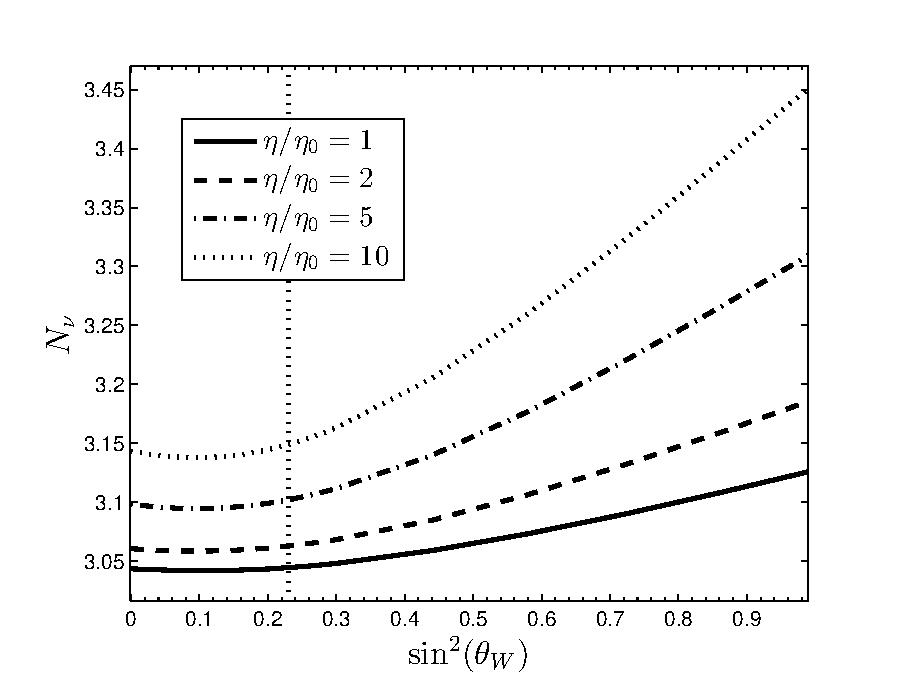
\includegraphics[width=0.70\columnwidth]{03-birrell/ParametricStudies/N_eff2.eps}
}
\caption{Change in effective number of neutrinos  $N_\nu$ as a function of Weinberg angle for  several values of $\eta/\eta_0=1,2,5,10$. Vertical line is $\sin^2(\theta_W)=0.23$.}
\label{N_nu_params}  
 \end{figure}
%%%%%%%%%%%%%%%%%%%%
We performed a least squares fit of $N_\nu$ over the range $0\leq \sin^2(\theta_W)\leq 1$, $1\leq \eta/\eta_0\leq 10$ shown in figure \ref{N_nu_params}, obtaining a result with relative error less than $0.2\%$,
\begin{align}
N_\nu=&3.003-0.095\sin^2\theta_W +0.222\sin^4\theta_W  -0.164\sin^6\theta_W \notag\\
+&\sqrt{\frac{\eta}{\eta_0}}\left(0.043+0.011\sin^2\theta_W +0.103\sin^4\theta_W\right).
\end{align}
$N_\nu$ is monotonically increasing in $\eta/\eta_0$ with dominant behavior  scaling as $\sqrt{ \eta/\eta_0}$. Monotonicity is to be expected, as increasing $\eta$ decreases the freeze-out temperature and the longer neutrinos are able to remain coupled to $e^\pm$, the more energy and entropy from annihilation is transferred to neutrinos.

We complement this with fits to the photon to neutrino temperature ratios $ T_\gamma / T_{\nu_e}, T_\gamma / T_{\nu_\mu}= T_\gamma / T_{\nu_\tau} $, and the neutrino fugacities, $\Upsilon_{\nu_e}, \Upsilon_{\nu_\mu}=\Upsilon_{\nu_\tau}$, again with relative error less than $0.2\%$  
\begin{align}
\frac{T_\gamma}{T_{\nu_\mu}}=&1.401+0.015x-0.040x^2+0.029x^3-0.0065y+0.0040xy-0.017x^2y, \label{fit1}\\
\Upsilon_{\nu_e}=&1.001+0.011x-0.024x^2+0.013x^3-0.005y-0.016xy+0.0006x^2y,\label{fit2}\\ 
\frac{T_\gamma}{T_{\nu_e}}=&1.401+0.015x-0.034x^2+0.021x^3-0.0066y-0.015xy-0.0045x^2y,\label{fit3}\\
\Upsilon_{\nu_\mu}=&1.001+0.011x-0.032x^2+0.023x^3-0.0052y+0.0057xy-0.014x^2y.\label{fit4}
%N_\nu=&3.003-0.095x+0.222x^2-0.164x^3+0.043y+0.011xy+0.103x^2y
\end{align}
where
\begin{equation}%{align}
x\equiv \sin^2 \theta_W ,\qquad
y\equiv  \sqrt{\frac{\eta}{\eta_0}}.
\end{equation}%{align}

%%%%%%%%%%%%%%%%%%%%
\begin{figure}%[H]
\centerline{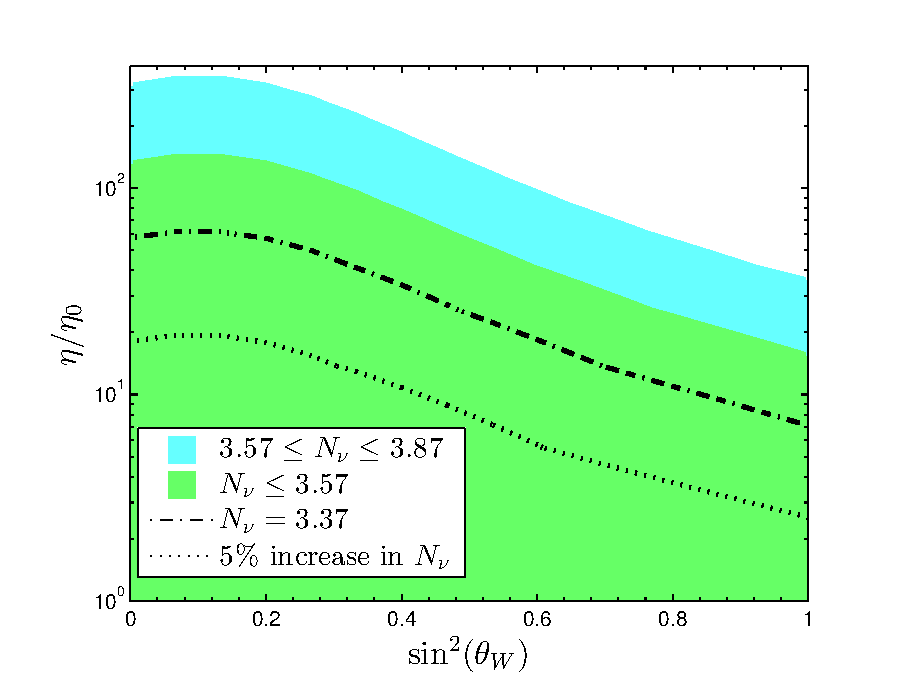
\includegraphics[width=0.75\columnwidth]{03-birrell/ParametricStudies/region_plot_legend.eps}
}
\caption{$N_\nu$ bounds in the $\eta/\eta_0, \sin^2(\theta_W)$ plane. Dark (green) for $N_\nu\in (3.03,3.57)$ corresponding to Ref.\cite{Planck} CMB+BAO analysis and light(teal) extends the region to $N_\nu<3.87$ i.e. to CMB+$H_0$. Dot-dashed line delimits the 1s.d. lower boundary of the second analysis.}
\label{N_nu_domain}
 \end{figure}
%%%%%%%%%%%%%%%%%%%%
The bounds on $N_\nu$ from the Planck analysis \cite{Planck} can be  used to constrain time or temperature variation of $\sin^2\theta_W$ and $\eta$.  
In  Figure \ref{N_nu_domain} the dark (green) color shows the combined range of  variation of natural constants  compatible with CMB+BAO and the light (teal) color shows  the extension in the range of  variation of  natural constants for CMB+$H_0$, both at a $68\%$ confidence level. The dot-dashed line within the dark (green) color  delimits   this latter domain. The dotted line shows the limit of a 5\% change in $N_\nu$.    Any increase in  $\eta/\eta_0$ and/or $\sin^2(\theta_W)$ moves the value of $N_\nu$ into the domain favored by current experimental results. Further parameter study is found in \ref{app:weinberg} and \ref{app:int_strength}.

%%%%%%%%%%%%%%%%%%%%
%%%%%%%%%%%%%%%%%%%%

%%%%%%%%%%%%%%%%%%%%
\subsection{Summary, Discussion, and Conclusions}\label{sec:concl}
We have employed a novel spectral method Boltzmann solver and a new procedure for evaluating the Boltzmann scattering integrals in order to characterize the impact of a potential time and/or temperature variation of SM parameters on the effective number of neutrinos. Specifically, we identified a dimensionless combination of $m_e$, $M_p$, and $G_F$, called the interaction strength $\eta$, that, along with the Weinberg angle $\sin^2 \theta_W$, control neutrino freeze-out and the resulting value of the effective number of neutrinos, $N_\nu$.  
%%%%%%%%%%%%%%%%%%%%%%%%%%%%%%%%%%%%%%%%%%%%%%%%%

%%%%%%%%%%%%%%%%%%%%%%%%%%%%%%%%%%%%%%%%%%%%%%%%%
\subsubsection{Primordial Variation of Natural Constants}
The question which we addressed in this section is: What neutrino decoupling in the early Universe can tell us about the values of natural constants when the Universe was about one second old and at an ambient temperature near to 1 MeV (11.6 billion degrees K). Our results were presented assuming that the Universe contains no other effectively massless particles but the three left handed neutrinos and corresponding, three right handed anti-neutrinos. 

We found that near to the physical value of the Weinberg angle  $\sin^2 \theta_W\simeq 0.23$ the effect of changing $\sin^2\theta_W$ on the decoupling of neutrinos is small. Thus as seen in Figure \ref{N_nu_params}  the dominant variance is due to the change  in the coupling strength $\eta/\eta_0$, \req{eta_def}  and \req{eta0_def}. The dotted line in  Figure \ref{N_nu_domain} shows that in order to achieve a change in $N_\nu$ at the level of up to 5\% that is  $N_\nu\lesssim 3.2 $  both $\sin^2 \theta_W$ and $\eta/\eta_0$ must change significantly, with e.g. $\eta$ increasing by an order of magnitude.

Let us look closer at what an increase in the strength parameter $\eta$ by factor 10 means, looking case by case on all the natural constant contributions as if each were responsible for the entire change:
\begin{itemize}
\item 
Considering that  $\eta\propto M_p\propto G_N^{-1/2}$ this translates into a decrease  in the strength of Gravity at neutrino freeze-out by a factor 100.  This effect would need to become much smaller by the time the age of the Universe is 1000 times longer (1s compared to 10 min) for Big Bang nucleosynthesis to be unaffected. This presumably means that, conversely, as we go further back in time we would need the gravity to continue to rapidly become very much weaker yet. In models of emergent gravity we can  imagine a  `melting' of gravity in the hot primordial Universe. Whether such a model can be realized will be a topic for future consideration. The attractive aspect of Gravity weakening rapidly with increasing temperature is that for  exponentially disappearing $G_N\to 0$ as $t\to 0$ and/or $T\to \infty$ the dynamics can be arranged to be similar to an inflationary  Universe.
\item 
Since $\eta\propto m_e^3$ electron mass would need to go up `only' by factor 2.15 . Compared to all other particles the electron mass has an anomalously  low value. Appearance of a mechanism just when $T\simeq m_e$ that `restores' the electron mass to where intuition would like it to be, a few MeV, arising from  the systematics of other Yukawa Higgs coupling $g_{Ye}$ compared to the Yukawa coupling of other charged light particles, where $m_e= g_{Ye} v $ seems to us also  a possible scenario. Interestingly,   laboratory limits for these conditions could be attainable in the foreseeable future.
\item
Since $\eta\propto G_F^2\propto 1/v^4$  we would need to find a mechanism that would decrease the vacuum value $v_0\simeq 246$ GeV by factor 1.8 already at temperature $T\simeq m_e$.  Allowing three powers of $v$ to cancel by using the Higgs minimal coupling formula for electron mass  we need to change $v$ by an order of magnitude near to $T\simeq m_e$. This appears impossible.
\end{itemize}
While ideas justifying strong variation of $\eta$ can be developed as two of the above three cases argue, a model for temperature or time dependence of  $\sin^2 \theta_W$ seems at this time without a theoretical anchor point, mainly so since we do not have a valid grand unified theoretical framework in which the electro-weak mixing or equivalently the masses $M_W, M_Z$ would be anchored.


%%%%%%%%%%%%%%%%%%%%%%%%%%%%%%%%%%%%%%%%%%%%%%%%%
\subsubsection{Two Different Ways to Change $N_\nu$}

However, there are additional challenges we have not at this time addressed. This is so since the immediate observable is the energy content of the invisible Universe as defined by the effective number of neutrinos $N_\nu$. Considering a value of   $N_\nu>3$,  there could  be a contribution from presently not discovered, more weakly interacting massless particles that decoupled even before neutrinos, and which therefore could contribute fractionally to $N_\nu$, see our discussion in Ref.\cite{Birrell:2014connect}. 

Of particular relevance could be a so called light sterile neutrino~\cite{Abazajian:2012ys}, possibly the right handed complement to the left handed neutrinos. If such particles exist and freeze-out well before regular neutrinos, their contribution to $N_\nu$ would be subject to dilution by reheating~\cite{Birrell:2014connect} and thus their contribution to $N_\nu$ would depend on when precisely they begin free-streaming.

These unknown dark `radiation' particles as well as neutrinos could have a mass that is at the scale of the temperature of photon decoupling $T_{\gamma 0}=0.25$ eV, for which an analysis of the Universe density fluctuations akin to Planck~\cite{Planck} would need to be adapted. We have  discussed in Ref.\cite{Birrell:2013_2} a consistent treatment of neutrino mass and $N_\nu$,  in the case of a particular type of delayed massive neutrino  freeze-out. This approach is exactly the same as would be the case for dark radiation:  Near to $T_{\gamma 0}=0.25$ eV massive neutrinos are indistinguishable from massive dark radiation, which contributes as an additional particle with reduced contribution to $N_\nu$~\cite{Birrell:2014connect}.

The alternative explanation of $N_\nu>3$ in terms of variation of  of natural constants that we have presented comprises  speculative beyond the standard model ideas akin in this aspect to new dark `radiation' particles. We believe that our present contribution provides a viable alternative  mechanism  capable of influencing $N_\nu$. In order to achieve an increase in $N_\nu$ the change in natural constants must cause a delay in neutrino freeze-out and thus  a greater participation of neutrinos in reheating during $e^\pm$ annihilation. The changes in the natural constants  which are required to make a large and visible contribution in $N_\nu$ appear at first sight to reach beyond a variation that one could tolerate at the time of big bang nucleosynthesis only a factor 1000 in time later. We have argued that a change in the electron mass $m_e$ by factor larger than two, and/or Newtons constant $G_N$ even by several orders of magnitude  could be present.




\subsection{Weinberg Angle Plots}\label{app:weinberg}



%%%%%%%%%%%%%%%%%%%%%%%%%%%%%%%%%%%%%%%
\begin{figure}[H]
\centerline{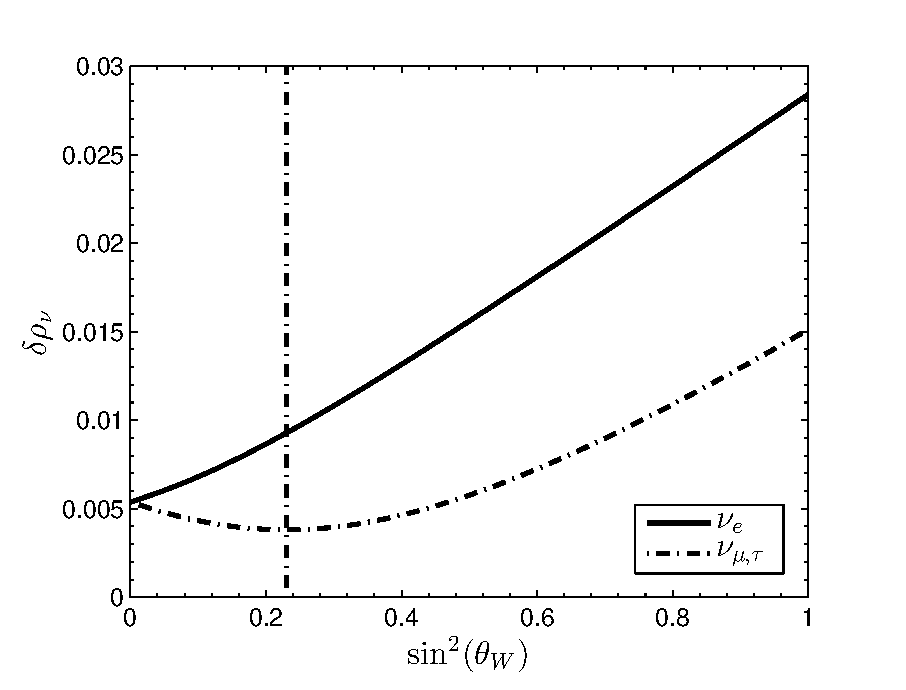
\includegraphics[height=5.8cm]{03-birrell/ParametricStudies/delta_rho.eps}\hspace{-5mm}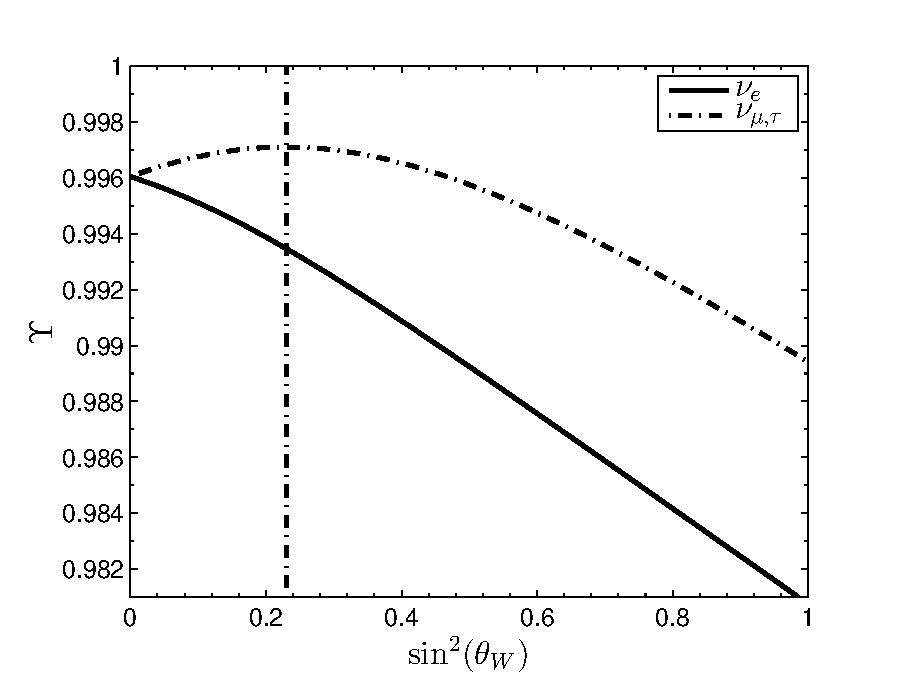
\includegraphics[height=5.8cm]{03-birrell/ParametricStudies/upsilon.eps}}
\caption{Fractional increase in neutrino energy (left) and neutrino fugacities (right), as functions of Weinberg angle. Vertical line is $\sin^2(\theta_W)=0.23$.}
 \end{figure}
%%%%%%%%%%%%%%%%%%%%%%%%%%%%%%%%%%%%%%%




%%%%%%%%%%%%%%%%%%%%%%%%%%%%%%%%%%%%%%
\begin{figure}[H]
\centerline{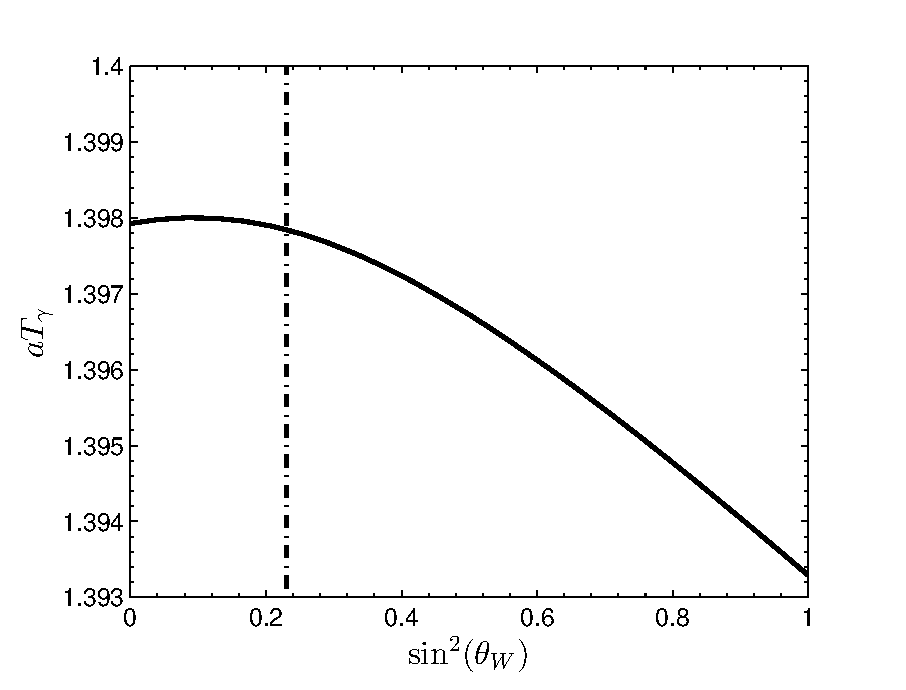
\includegraphics[height=5.8cm]{03-birrell/ParametricStudies/aT_gamma.eps}\hspace{-5mm}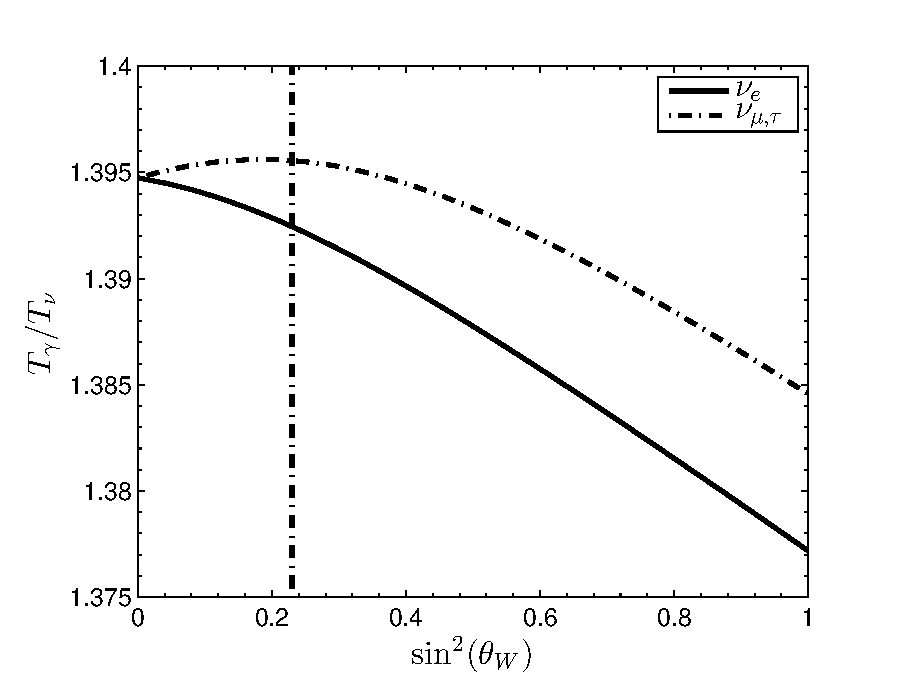
\includegraphics[height=5.8cm]{03-birrell/ParametricStudies/T_ratio.eps}}
\caption{Dependence on Weinberg angle of photon reheating  (left) and photon-neutrino temperature ratios (right) after freeze-out. Vertical line is $\sin^2(\theta_W)=0.23$.}
 \end{figure}
%%%%%%%%%%%%%%%%%%%%%%%%%%%%%%%%%%%%%%%



%%%%%%%%%%%%%%%%%%%%%%%%%%%%%%%%%%%%%%%
\begin{figure}[H]
\centerline{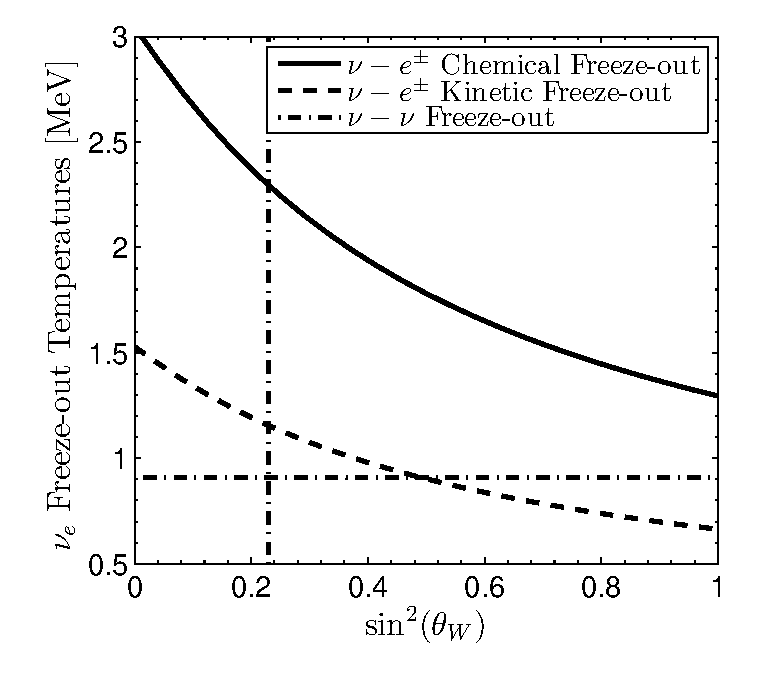
\includegraphics[height=6.3cm]{03-birrell/ParametricStudies/nu_e_freezeout.eps}\hspace{5mm}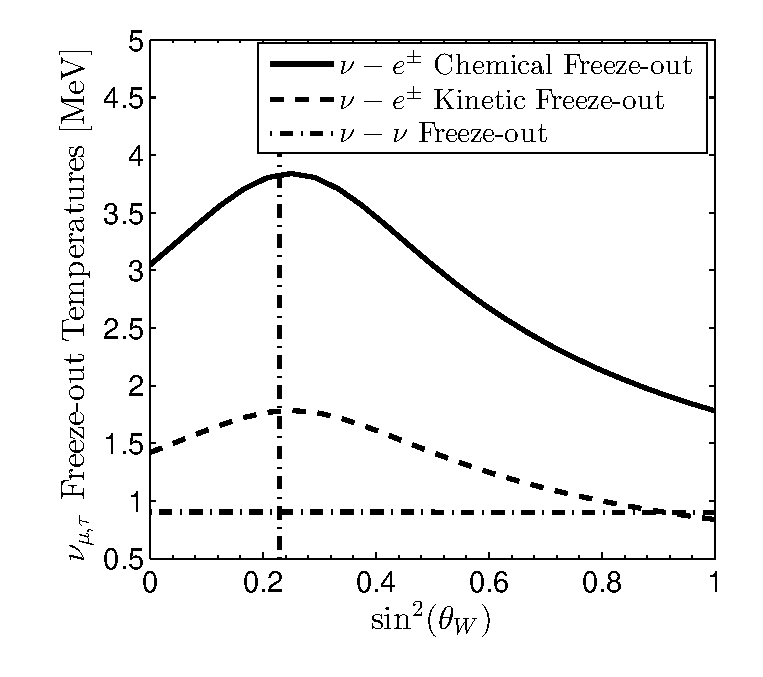
\includegraphics[height=6.3cm]{03-birrell/ParametricStudies/nu_mu_freezeout.eps}}
\caption{Freeze-out temperatures for electron neutrinos (left) and $\mu$, $\tau$ neutrinos (right) for various types of processes, as functions of Weinberg angle. Vertical line is $\sin^2(\theta_W)=0.23$.}\label{fig:freezeoutT}
 \end{figure}
%%%%%%%%%%%%%%%%%%%%%%%%%%%%%%%%%%%%%%%

\subsection{Interaction Strength Plots}\label{app:int_strength}



%%%%%%%%%%%%%%%%%%%%%%%%%%%%%%%%%%%%%%%
\begin{figure}[H]
\centerline{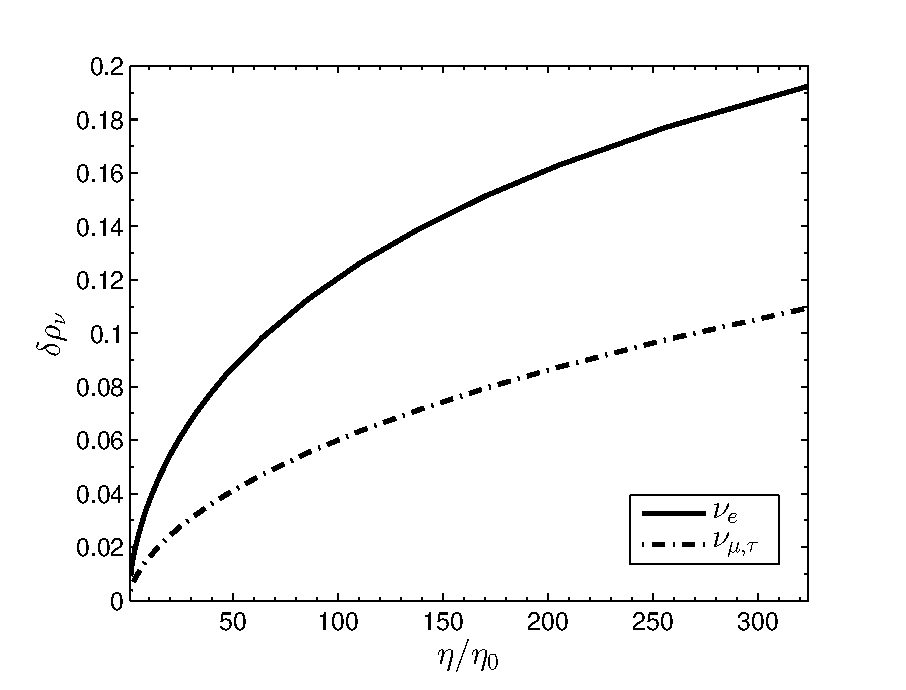
\includegraphics[height=5.8cm]{03-birrell/ParametricStudies/delta_rho_GF.eps}\hspace{-5mm}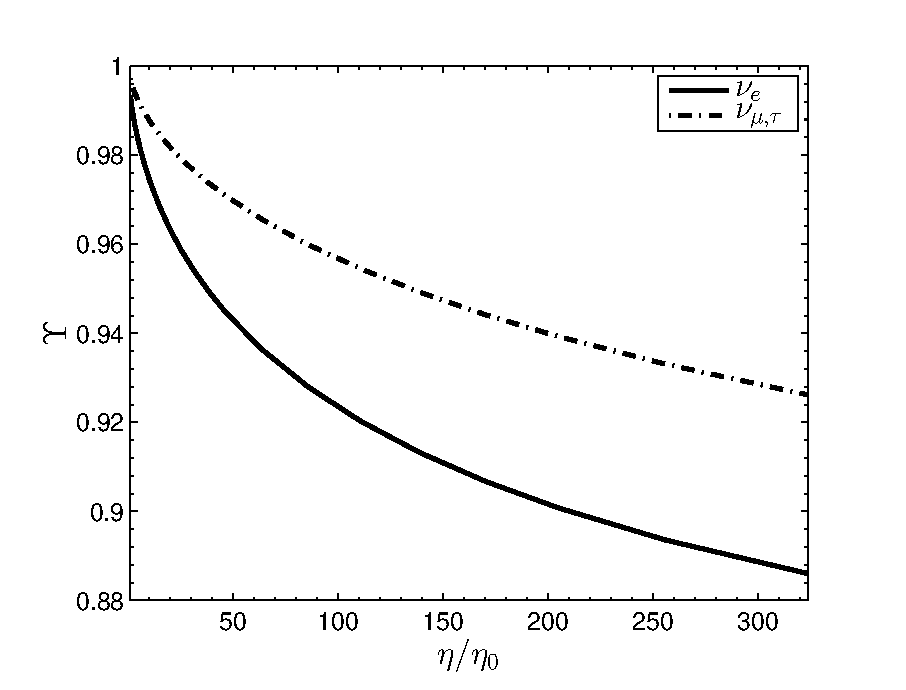
\includegraphics[height=5.8cm]{03-birrell/ParametricStudies/upsilon_GF.eps}}
\caption{Fractional increase in neutrino energy (left) and neutrino fugacities (right), as functions of interaction strength.}
 \end{figure}
%%%%%%%%%%%%%%%%%%%%%%%%%%%%%%%%%%%%%%%




%%%%%%%%%%%%%%%%%%%%%%%%%%%%%%%%%%%%%%
\begin{figure}[H]
\centerline{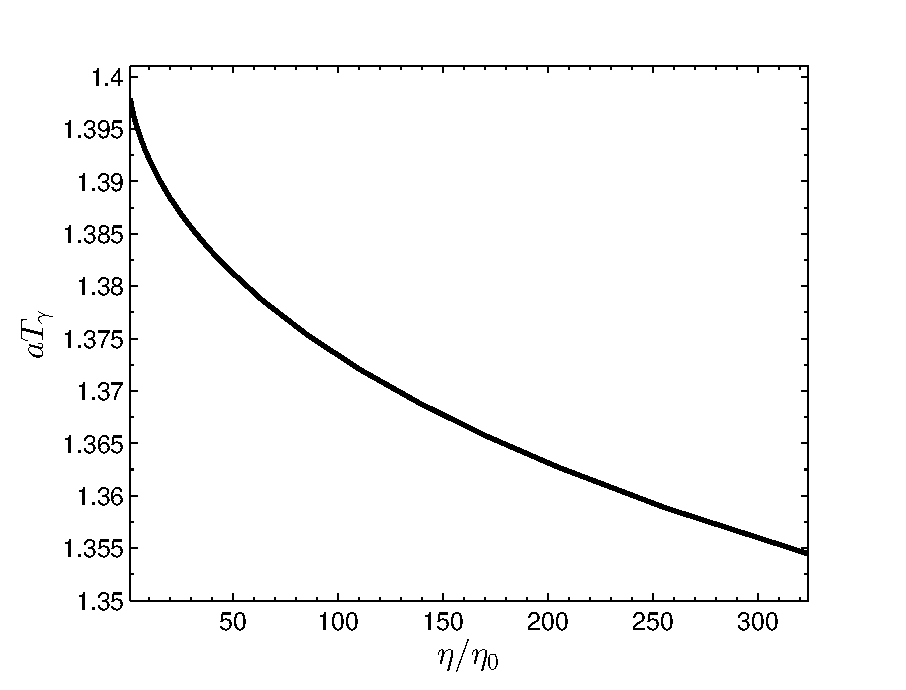
\includegraphics[height=5.8cm]{03-birrell/ParametricStudies/aT_gamma_GF.eps}\hspace{-5mm}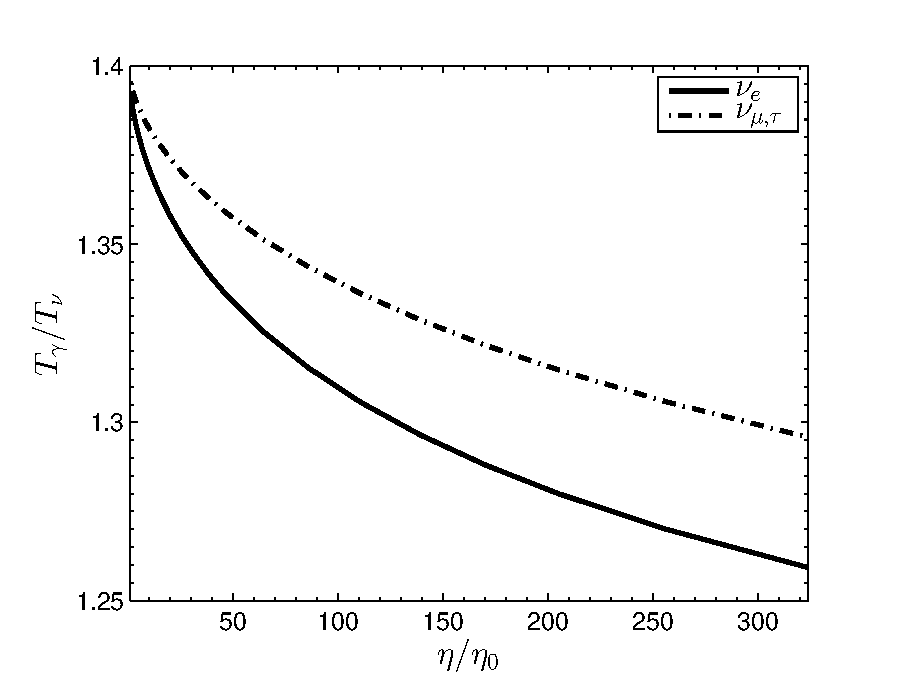
\includegraphics[height=5.8cm]{03-birrell/ParametricStudies/T_ratio_GF.eps}}
\caption{Dependence on  interaction strength of photon reheating (left) and photon-neutrino temperature ratios (right) after freeze-out.}
 \end{figure}
%%%%%%%%%%%%%%%%%%%%%%%%%%%%%%%%%%%%%%%



%%%%%%%%%%%%%%%%%%%%%%%%%%%%%%%%%%%%%%%
\begin{figure}[H]
\centerline{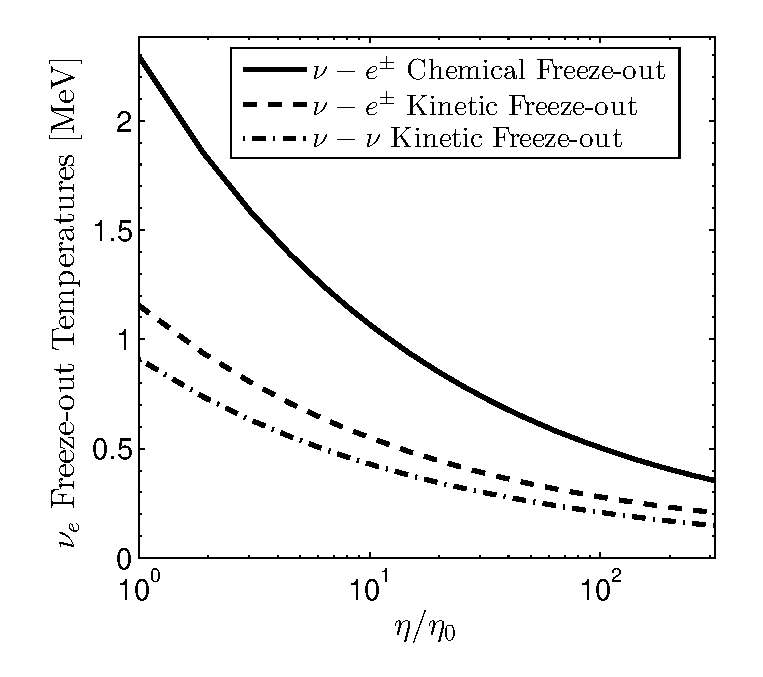
\includegraphics[height=6.3cm]{03-birrell/ParametricStudies/nu_e_freezeout_GF.eps}\hspace{5mm}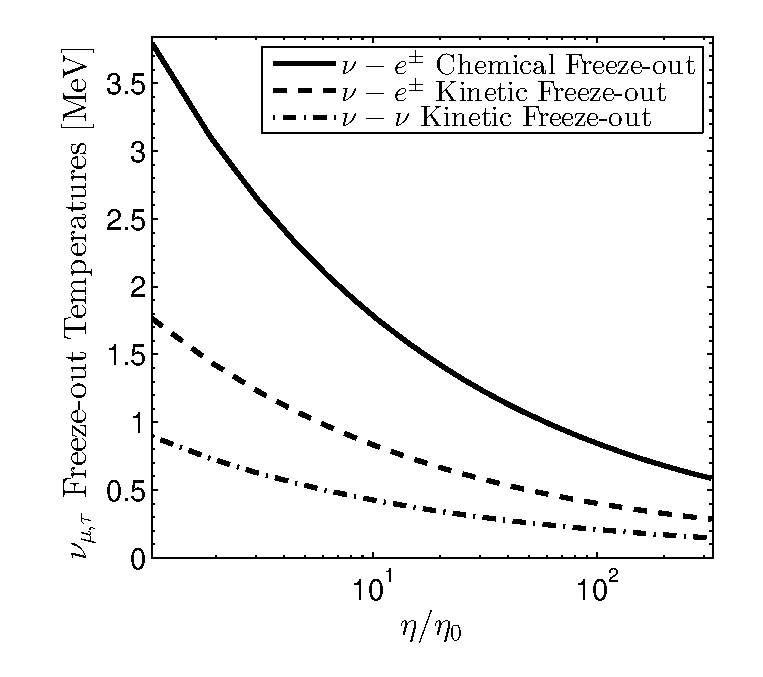
\includegraphics[height=6.3cm]{03-birrell/ParametricStudies/nu_mu_freezeout_GF.eps}}
\caption{Freeze-out temperatures for electron neutrinos (left) and $\mu$, $\tau$ neutrinos (right) for various types of processes, as functions of interaction strength.}
 \end{figure}
%%%%%%%%%%%%%%%%%%%%%%%%%%%%%%%%%%%%%%%


